\documentclass{standalone}
\usepackage{tikz}
\usetikzlibrary{arrows.meta,positioning,calc}
\begin{document}
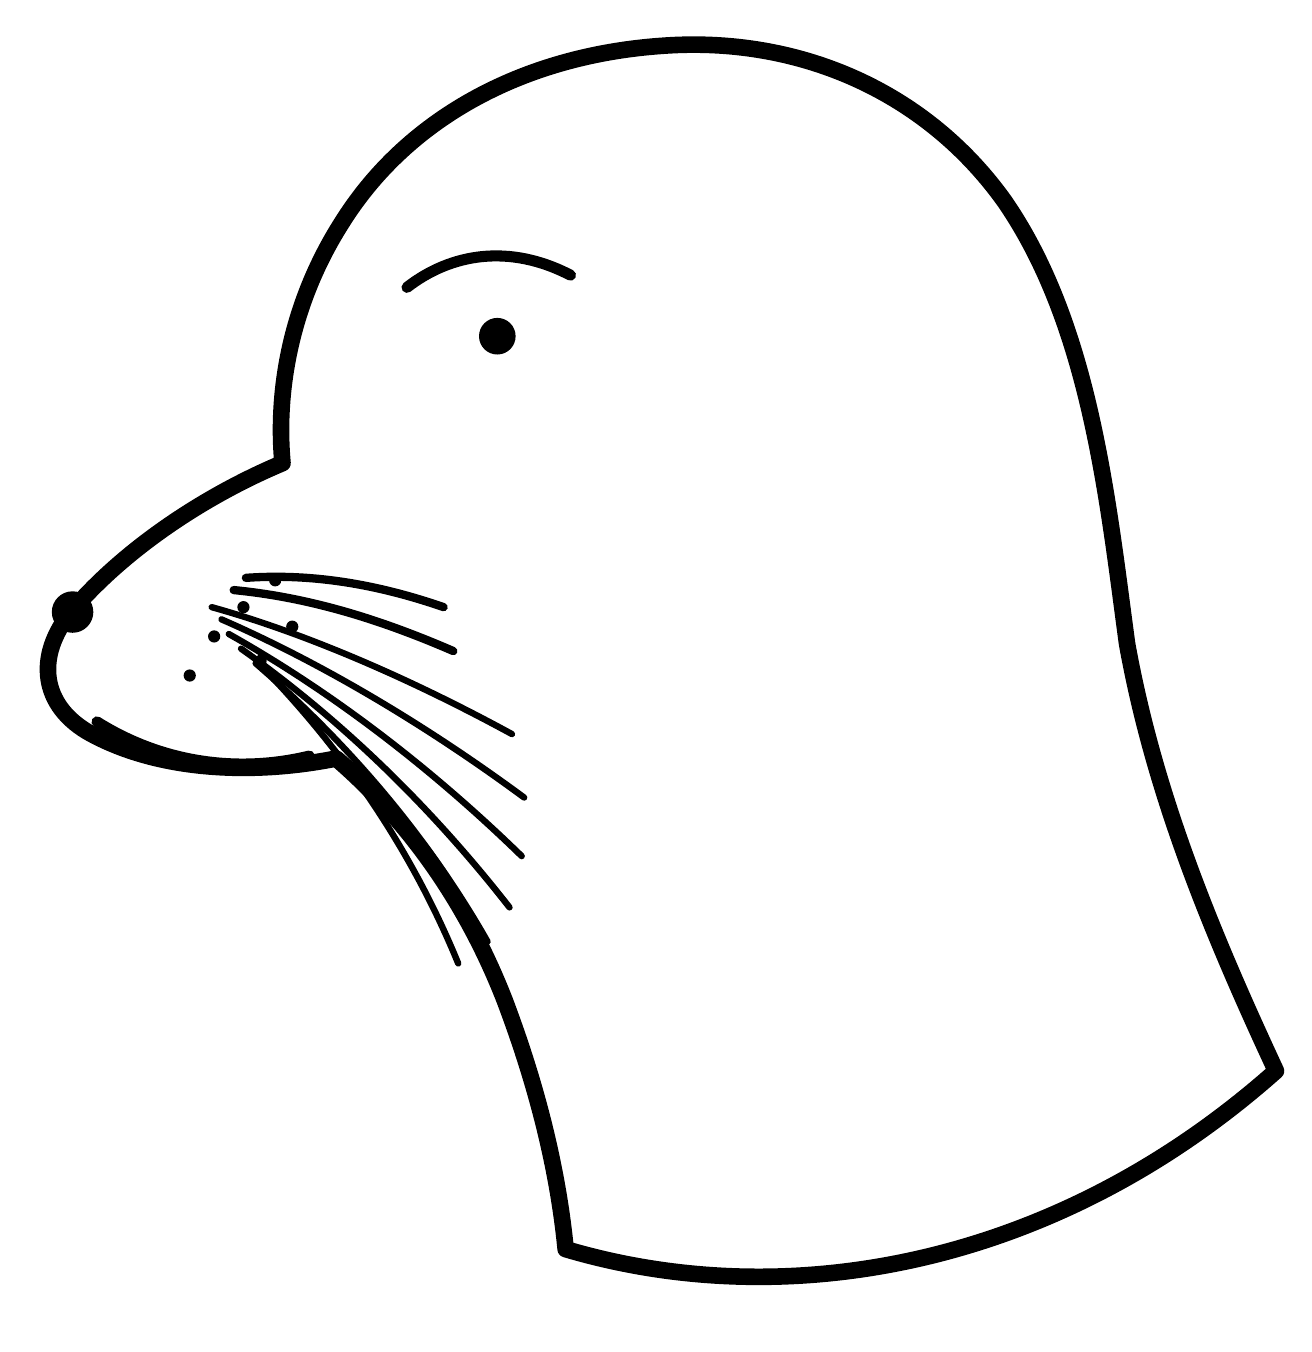
\begin{tikzpicture}[
  x=1cm,
  y=1cm,
  scale=3.1,
  line cap=round,
  line join=round
]

% Draw the seal facing left.
% The QR code is outside this mirrored scope.
\begin{scope}[xscale=-1]

% Head and neck outline
\draw[line width=6pt]
  (-1.65,-1.70)
  .. controls (-1.38,-1.12) and (-1.15,-0.56) ..
     (-1.04,0.05)
  .. controls (-0.96,0.64) and (-0.89,1.35) ..
     (-0.54,1.86)
  .. controls (-0.22,2.31) and (0.30,2.54) ..
     (0.86,2.50)
  .. controls (1.45,2.46) and (1.92,2.19) ..
     (2.18,1.77)
  .. controls (2.37,1.47) and (2.45,1.12) ..
     (2.42,0.79)
  .. controls (2.73,0.66) and (3.05,0.45) ..
     (3.27,0.20)
  .. controls (3.43,0.02) and (3.42,-0.19) ..
     (3.22,-0.31)
  .. controls (2.94,-0.47) and (2.55,-0.49) ..
     (2.20,-0.42)
  .. controls (1.91,-0.67) and (1.67,-1.00) ..
     (1.51,-1.41)
  .. controls (1.37,-1.78) and (1.29,-2.12) ..
     (1.26,-2.43)
  .. controls (0.35,-2.70) and (-0.75,-2.50) ..
     (-1.65,-1.70)
  -- cycle;

% Nose
\fill (3.28,0.18) circle (0.085);

% Eye
\fill (1.54,1.31) circle (0.075);

% Brow
\draw[line width=4pt]
  (1.24,1.56)
  .. controls (1.49,1.69) and (1.73,1.65) ..
     (1.91,1.51);

% Mouth
\draw[line width=4pt]
  (3.18,-0.27)
  .. controls (2.91,-0.44) and (2.60,-0.48) ..
     (2.31,-0.41);

% Muzzle dots
\foreach \x/\y in {
  2.45/0.31,
  2.58/0.20,
  2.38/0.12,
  2.70/0.08,
  2.51/-0.02,
  2.80/-0.08
}{
  \fill (\x,\y) circle (0.025);
}

% Whiskers point toward the neck in this unmirrored
% coordinate system. The scope then mirrors them correctly.
\draw[line width=2.3pt]
  (2.71,0.20)
  .. controls (2.35,0.10) and (1.92,-0.08) ..
     (1.48,-0.32);

\draw[line width=2.3pt]
  (2.67,0.15)
  .. controls (2.28,-0.02) and (1.85,-0.27) ..
     (1.43,-0.58);

\draw[line width=2.3pt]
  (2.64,0.09)
  .. controls (2.23,-0.14) and (1.82,-0.45) ..
     (1.44,-0.82);

\draw[line width=2.3pt]
  (2.59,0.03)
  .. controls (2.18,-0.26) and (1.81,-0.62) ..
     (1.49,-1.03);

\draw[line width=2.3pt]
  (2.53,-0.03)
  .. controls (2.16,-0.35) and (1.83,-0.73) ..
     (1.58,-1.17);

\draw[line width=2.3pt]
  (2.46,-0.09)
  .. controls (2.14,-0.43) and (1.88,-0.82) ..
     (1.70,-1.26);

% Short upper whiskers
\draw[line width=3pt]
  (2.62,0.27)
  .. controls (2.31,0.24) and (2.02,0.15) ..
     (1.72,0.02);

\draw[line width=3pt]
  (2.57,0.32)
  .. controls (2.29,0.34) and (2.02,0.29) ..
     (1.76,0.20);

\end{scope}

\end{tikzpicture}
\end{document}
